%===============================================================================
% SECTION: METHODS
%===============================================================================
\section{RAPTORGraph: model architecture and learning}
\label{sec:methods}
%===============================================================================

\gls{raptorgraph} is an end-to-end framework designed to learn causal relationships from interventional single-cell data (Perturb-seq data). It consists of two novel modules: a preconditioned GraphPathway Encoder~(\cref{subsec:methods:graphpathway}) that maps genes to learned interpretable causal latent factors (the \cmps{})  and a DAGMA-based DAG module~(\cref{subsec:methods:dagma}) that infers the causal graph between the learnt \cmps{}.
The proposed design directly addresses the Intervention Spillover Problem ensuring by construction, ensuring that gene interventions target a unique \cmp{}.
We refer to \cref{app:architecture:overview} for a  detailed description  of the model.

%-------------------------------------------------------------------------------
% Subsection: GraphPathway Encoder for Deconfounding through Preconditioning
%-------------------------------------------------------------------------------
\subsection{GraphPathway encoder with preconditioning}
\label{subsec:methods:graphpathway}
%-------------------------------------------------------------------------------

To address the Intervention Spillover Problem and enforce the theoretical requirement for single-causal-factor interventions, we introduce a novel encoder architecture, the GraphPathway Encoder, which features a deconfounding approach through preconditioning.
This approach requires a specific ordering of the input data.
Let $\numperturbedgenes$ be the number of known perturbed genes in the experiment.
Without loss of generality, we assume the input gene vector $\variables \in \realnumbers^\observeddim$ is sorted such that the first $\numperturbedgenes$ genes are those perturbed, followed by the remaining $\observeddim-\numperturbedgenes$ unperturbed genes.

\textbf{Pre-conditioning module (\cref{fig:arch:graphpathway_encoder}-A)}. Given this sorted input, we define our model with $\latentdim$ learned \cmps{}, where we require that the number of learned \cmps{} is at least the number of perturbed genes ($\latentdim \ge \numperturbedgenes$).
We then structure the encoder's primary weight matrix $\weightmatrix$ as a block matrix that enforces a sparse, one-to-one mapping for perturbed genes while allowing dense interactions for the unperturbed components (see \cref{app:graphpathway} for the formal definition of $\weightmatrix$).

This diagonal structure ensures each of the $\numperturbedgenes$ perturbed genes directly influences only one of the first $\numperturbedgenes$ learned \cmps{} (\cref{fig:arch:graphpathway_encoder}-\textbf{A}).
The zero block in $\weightmatrix$ is critical for preventing intervention spillover by explicitly blocking the influence of perturbed genes on the remaining learned \cmps{}.
The other submatrices are learnable and dense, allowing the model flexibility to discover complex gene-gene relationships across all unperturbed genes and learned \cmps{}.

Crucially, this preconditioned structure allows the intervention mask $\maskvector$, which specified which \cmp{} to shift for each intervention, to be predefined and fixed rather than learned, thereby satisfying the key structural requirements for identifiability.

\textbf{Latent grouping via an interaction block (\cref{fig:arch:graphpathway_encoder}-B)}. To model the complex non-linear gene-gene dynamics of biological systems, our architecture extends the preconditioning by learning multiple distinct subgraph representations for each meta-pathway.
An intermediate \emph{Interaction Block} then processes these subgraph activations, allowing the model to capture higher-order dependencies by learning unique interaction patterns among the subgraphs within each learned meta-pathway (\cref{fig:arch:graphpathway_encoder}-\textbf{B}).

\textbf{Meta-pathway inference via VAE (\cref{fig:arch:graphpathway_encoder}-C)}. Next, an aggregation layer combines these processed features to compute the VAE parameters ($\vect{\mu}_{\latentvars}$ and $\vect{\sigma}_{\latentvars}$) for the meta-pathway distributions (\cref{fig:arch:graphpathway_encoder}-\textbf{C}). Thus, the final stochastic representations of the meta-pathways are then obtained using the reparameterization trick $\latentvars = \vect{\mu}_{\latentvars} + \vect{\sigma}_{\latentvars} \circ \vect{\epsilon}; \quad \vect{\epsilon} \sim \normaldist(\vect{0}, \identitymatrix)$.

\revised{\textbf{\cmp{} inference via DAGMA (\cref{fig:arch:graphpathway_encoder}-D, \cref{subsec:methods:dagma})}. The model then represents the downstream biological consequences of genetic interventions through the activities of \cmps{}. Specifically, a DAGMA layer propagates the VAE-learned (independent) meta-pathway activities through a learned directed acyclic graph, yielding the final causally dependent meta-pathway activities.}

As last step of the model, a non-linear dense decoder maps these causal states back to the high-dimensional gene expression space to predict the post-perturbation (or unperturbed/control) gene expression. 
For a comprehensive architectural description, we refer the reader to \cref{app:graphpathway}.

\begin{figure}[t]
    \centering
    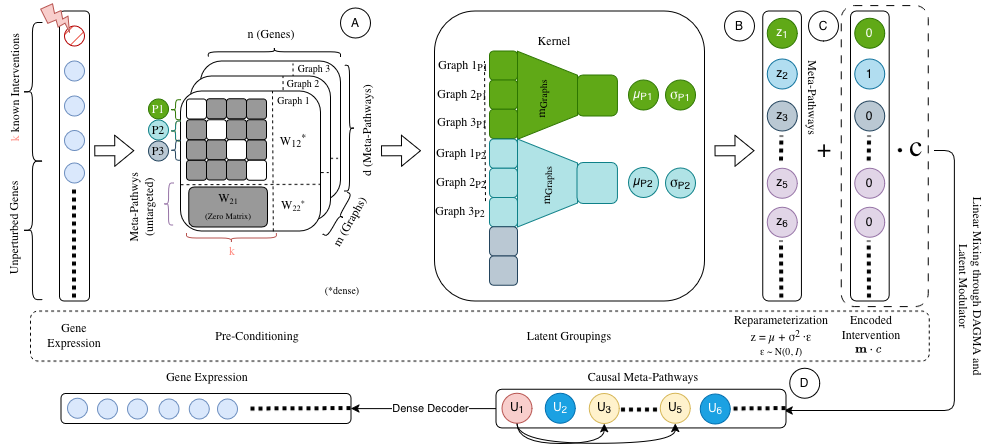
\includegraphics[width=\linewidth]{gfx/GraphPathway_modified.png}
    \caption{
        \textbf{The GraphPathway Encoder architecture of \gls{raptorgraph}.}
        \textbf{A}: \revised{Gene expression of control cells ($\zobs$) is fed as input to} the preconditioned linear layer, \revised{which} enforces a sparse, one-to-one mapping for known perturbed genes \revised{to explicitly} prevent intervention spillover.
        \textbf{B}: \revised{Complex dependencies are captured by learning} multiple parallel graph representations, \revised{which are then} aggregated to model non-linear interactions.
        \textbf{C}: A standard \gls{vae} reparameterization head \revised{generates} the stochastic latent variables \revised{($\latentvars$)}.
        \textbf{D}: A \revised{Latent Modulator takes the perturbation label as input and applies} atomic perturbations \revised{($\effectvector$)} to the independent latents \revised{($\latentvars$), shifting the distribution from the observed latent state ($\zobs$) to the interventional latent state ($\zint$). Both $\zobs$ and $\zint$ are then transformed by the DAGMA layer} through the learned \gls{dag} via linear mixing to \revised{yield} the final causal states \revised{($\latentcausalvars$), which are reconstructed into the predicted control ($\hat{\variables}_{\text{obs}}$) and perturbed ($\hat{\variables}_{\text{int}}$) gene expression profiles by a dense decoder.}
    }
    \label{fig:arch:graphpathway_encoder}
\end{figure}

% \begin{figure}[htbp]
%     \centering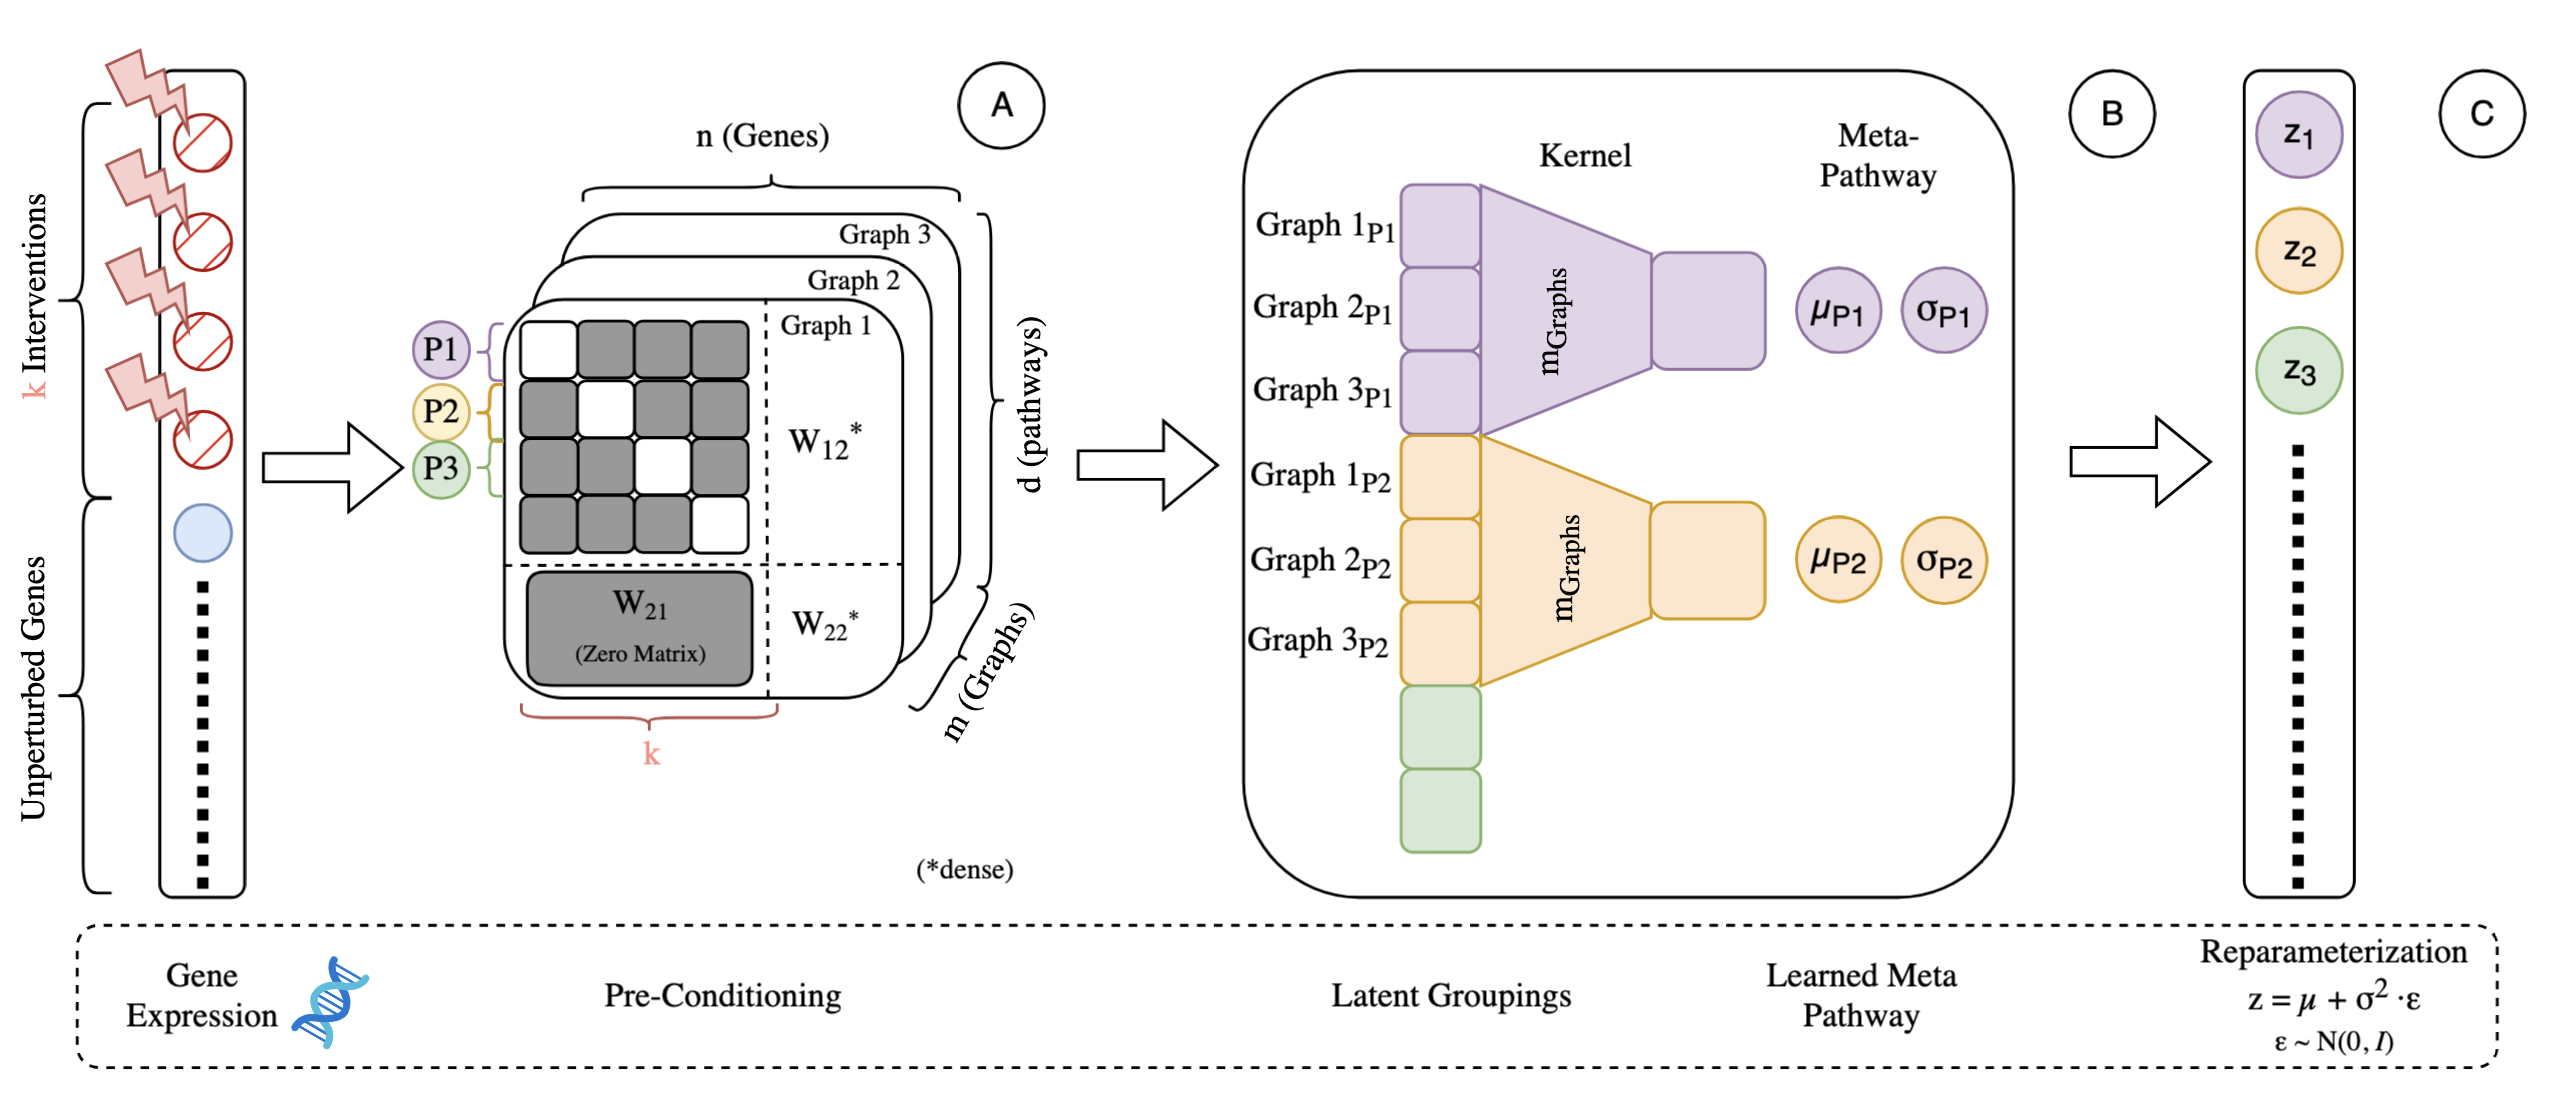
\includegraphics[width=1\linewidth]{gfx/GraphPathwayLayer_final.png}
%     \caption{
%         The GraphPathway Encoder architecture of \gls{raptorgraph}.
%         \textbf{A}: The preconditioned linear layer enforces a sparse, one-to-one mapping for known perturbed genes, preventing spillover.
%         \textbf{B}: Multiple parallel graph representations are learned and then aggregated to model non-linear interactions.
%         \textbf{C}: A standard \gls{vae} reparameterization head produces the final stochastic latent variables.
%     }\label{fig:arch:graphpathway_encoder}
% \end{figure}

%-------------------------------------------------------------------------------
% Subsection: Deep Causal Graph Learning with DAGMA
%-------------------------------------------------------------------------------
\subsection{Deep Causal Graph Learning with DAGMA}
\label{subsec:methods:dagma}
%-------------------------------------------------------------------------------

The GraphPathway Encoder with preconditioning fundamentally alters the causal structure discovery task.
By fixing the mapping  to specific latent variables, it eliminates the need for permutation-based discovery methods that assume a dense, entangled encoder.
However, this fixed ordering makes simple acyclicity constraints, such as enforcing an upper-triangular adjacency matrix, unsuitable.
These methods impose a strict and arbitrary causal hierarchy, as the influence of one latent variable on another is entirely restricted by their ordering (e.g., latent $i$ can only influence latent $j$ if $i<j$), which would conflict with the true biological relationships we aim to discover.
For this, we adapt the DAGMA framework~\citep{bello2022dagma} for its use in a deep learning context.

\textbf{DAGMA} reformulates the combinatorial search for a \gls{dag} into a continuous optimization problem.
This is achieved by minimizing a score function that measures data fit, subject to a differentiable constraint that is satisfied only if the graph is acyclic.
The DAGMA acyclicity constraint, $\acyclicityfunc_s(\graphmatrix)$, is based on a log-determinant function:
\begin{equation}
    \acyclicityfunc_s(\graphmatrix) = -\log\det(s\identitymatrix - \graphmatrix \circ \graphmatrix) + \latentdim\log s = 0
\end{equation}
where $\graphmatrix \in \realnumbers^{\latentdim \times \latentdim}$ is the weighted adjacency matrix of the latent graph, $s > 0$ is a scaling scalar, and $\circ$ represents the Hadamard product. Note that the condition holds if and only if $\graphmatrix$ represents a \gls{dag}.
The optimization then solves a sequence of unconstrained problems that jointly minimize a data-fit score and the acyclicity penalty.

%We implement a modified DAGMA approach with a dual-gradient system to ensure stability and causal fidelity.
%The causal graph is learned by computing the DAGMA loss exclusively on the latent representations of observational data.
%This encourages the model to learn the invariant, baseline causal structure of the biological system.
%Our implementation includes several key modifications for stable and effective graph discovery within a deep generative model.
\revised{\textbf{DAGMA implementation.} We implement a modified DAGMA approach designed to learn the invariant, baseline causal structure of the biological system.
To ensure stability and manage the trade-off between reconstruction fidelity and acyclicity, we introduce two critical regularization.
First, we employ a path-following schedule where the score weight $\mu$ is gradually decreased (see \cref{eq:dagma_loss_full}), allowing the model to prioritize feature learning early in training before strictly enforcing the graph constraint.
Second, we isolate gradient flow by computing the DAGMA-associated loss $\dagmaloss$ on detached latent representations.
This ensures the acyclicity constraint optimizes the graph structure without distorting the encoder's representation learning.}
A detailed description of the DAGMA layer, its objective, theoretical background, and implementation can be found in \cref{app:dagma}.

%===============================================================================
\subsection{Optimal Transport for Deterministic Interventional Learning}
%===============================================================================

A fundamental challenge in single-cell interventional modeling is the lack of direct one-to-one mappings between control and perturbed cells, creating a counterfactual gap.
Standard approaches often address this by randomly pairing control and interventional samples during training.
However, this random pairing matches cells with poor counterfactuals, providing inconsistent gradient signals that force the model to minimize loss by predicting the average of the target distribution---a phenomenon we term \textit{mean collapse} (see \cref{fig:app:ot_comparison}).
To resolve this, we employ a Wasserstein-based \gls{ot} framework to establish a deterministic, globally optimal mapping.
By minimizing the total transport cost between the control and perturbed populations, \gls{ot} pairs each cell with its most biologically similar counterpart.
This preserves heterogeneous subpopulation structures and ensures stable, structure-preserving representations for causal discovery.
Mathematical details are provided in \cref{app:ot}.

%-------------------------------------------------------------------------------
% Subsection: Training Objective
%-------------------------------------------------------------------------------
\subsection{Training Objective}
\label{subsec:methods:loss}
%-------------------------------------------------------------------------------

The model is trained end-to-end by minimizing a composite objective function, $\totalloss$, which balances four specialized components to ensure robust representation learning and causal discovery:
\begin{equation}
    \totalloss = \alpharec\mseloss + \betakl\kldloss +\quad \gammammd\mmdloss + \deltadagma\dagmaloss
    \label{eq:total_loss}
\end{equation}
where the scalar hyperparameters $\alpharec, \betakl, \gammammd$, and $\deltadagma$ balance each term's contribution. 
Specifically, we employ a reconstruction loss ($\mseloss$) to maintain high-fidelity control unperturbed cell reconstruction; 
a KL divergence ($\kldloss$) to regularize the meta-pathway manifold; 
an interventional prediction loss ($\mmdloss$) to align distributions of predicted perturbed gene expressions with those of the experimental ground truth; 
and a causal graph loss ($\dagmaloss$) to enforce structural acyclicity and data fit, defined as:
\begin{equation}
    \dagmaloss = \mu(\scorefunc(\graphmatrix; \datamatrix) + \lambda_1 \|\graphmatrix\|_1) + \acyclicityfunc(\graphmatrix)
    \label{eq:dagma_loss_full}
\end{equation}
where $\scorefunc(\graphmatrix; \datamatrix)$ is a score (see \cref{app:dagma:optimization}), $\|\graphmatrix\|_1$ is the L1 norm of the adjacency matrix, and $\acyclicityfunc(\graphmatrix)$ is the acyclicity penalty.
A comprehensive derivation and discussion of each term is provided in \cref{app:metrics}.
